\section{Circuito RLC in corrente impulsata}
In questa parte di esperienza abbiamo avuto come scopo quello di studiare l'andamento della differenza di potenziale ai capi delle componenti di un circuito RLC, sollecitato da un segnale ad onda quadra.

In primo luogo abbiamo montato il circuito come in figura, sollecitandolo da un segnale ad onda quadra:
\begin{figure} [H]
    \centering
    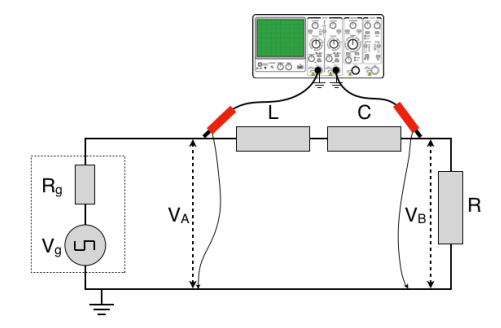
\includegraphics[scale=.9]{Immagini/Configurazione2.PNG}
    \label{fig:my_label}
    \caption{Configurazione circuito RLC}
\end{figure}

Successivamente abbiamo misurato il segnale di tensione ai capi della resistenza mediante una sonda, posta come indicato.


Per l'analisi del circuito abbiamo dimensionato la configurazione in modo da avere un regime sottosmorzato, uno sovrasmorzato e uno con smorzamento critico.


\subsection{Regime di sottosmorzato}
Nel caso sottosmorzato abbiamo scelto una frequenza tale da vedere nell'Oscilloscopio almeno 5 massimi e affinchè il terzo massimo di $V_{R}(t)$ sia non meno di $\frac{1}{10}$ dal primo. Di seguito, in Fig. \ref{fig: sottosmorzato}, viene esposto il grafico con relativo fit e vengono ricavati i parametri di interesse.
\begin{figure}[H]
    \centering
    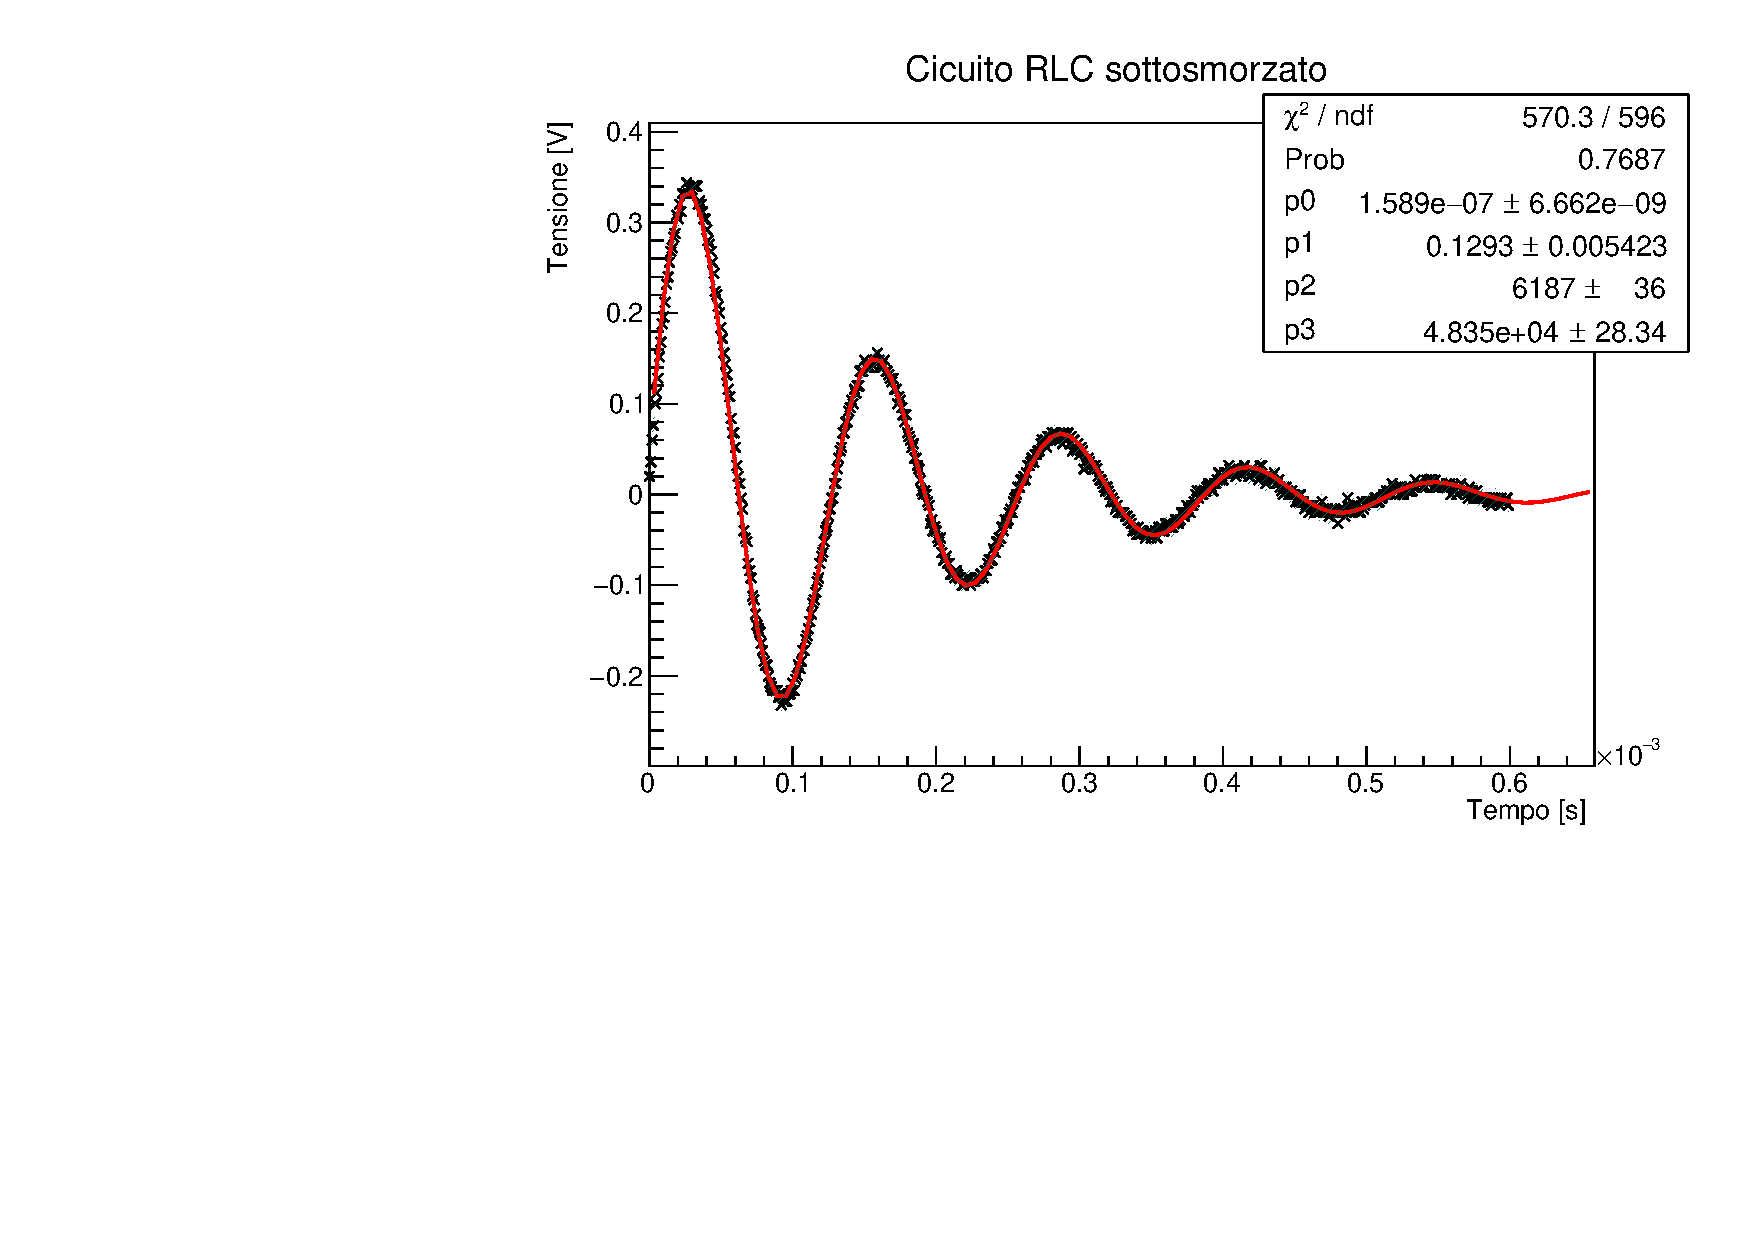
\includegraphics[scale=.4]{Immagini/Circuito_RLC_sottosmorzato.pdf}
    \caption{RLC sottosmorzato}
    \label{fig: sottosmorzato}
\end{figure}

\begin{table}[H]
    \centering
    \begin{tabular}{cc}
    \toprule
      Parametro   & Valore corrispondente \\
    \midrule
       p0  & $C$ \\
       p1  & $V_0$ \\
       p2  & $\gamma$ \\
       p3  & $\omega$ \\
    \bottomrule
    \end{tabular}
    \caption{}
\end{table}
Si ricava per cui che i parametri di tale circuito sono:
\begin{table}[h!]
    \centering
    \begin{tabular}{cc}
        \toprule
      $L (mH)$  & $C (F)$ \\
         \midrule
    $32,32\pm 1,63$     & $1,589\pm 6,67\times 10^{-3}$\\
    \bottomrule
    \end{tabular}
    \caption{}
\end{table}


\subsection{Regime di sovrasmorzamento}
Nel caso sovrasmorzato abbiamo scelto una frequenza tale da vedere nell'Oscilloscopio $V_{R}(t)$ almeno di $\frac{1}{10}$ del suo valore.
\begin{figure}[H]
    \centering
    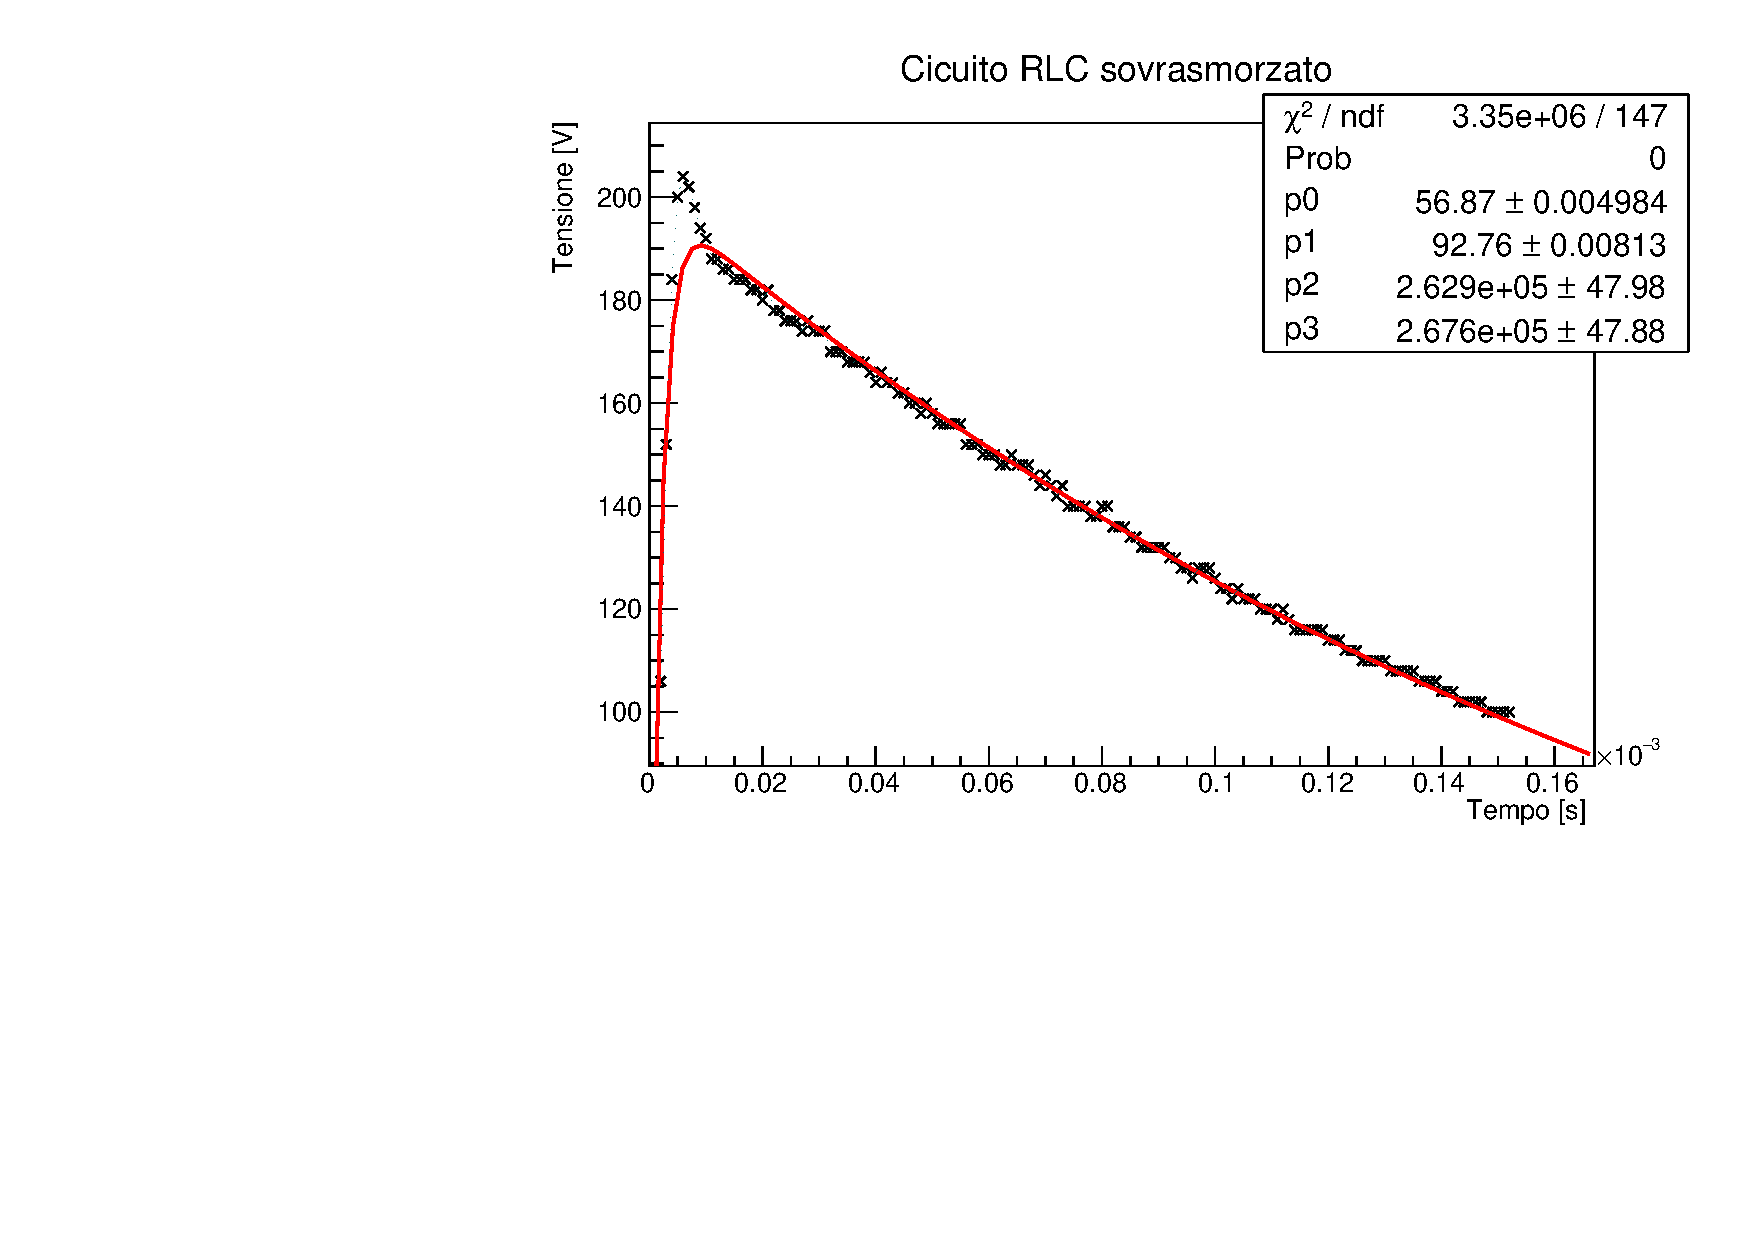
\includegraphics[scale=.4]{Immagini/Circuito_RLC_sovrasmorzato.pdf}
    \caption{RLC sovrasmorzato}
\end{figure}
\begin{table}[H]

    \centering
    \begin{tabular}{cc}
    \toprule
      Parametro   & Valore corrispondente \\
    \midrule
       p0  & $Q_0$ \\
       p1  & $\omega_0^2$ \\
       p2  & $\beta$ \\
       p3  & $\gamma$ \\
    \bottomrule
    \end{tabular}
    \caption{}
\end{table}
Si ricava per cui che i parametri di tale circuito sono:
\begin{table}[h!]
    \centering
    \begin{tabular}{cc}
        \toprule
      $L (mH)$  & $C (mF)\times 10^{-7}$ \\
         \midrule
    $37,37 \pm 1,86$     & $288,48\pm 0,51$\\
    \bottomrule
    \end{tabular}
    \caption{}
\end{table}

\subsection{Regime smorzamento critico}
Come nel caso di regime sovrasmorzato, per lo smorzamento critico abbiamo scelto una frequenza tale da vedere nell'Oscilloscopio $V_{R}(t)$ almeno di $\frac{1}{10}$ del suo valore.
\begin{figure}[H]
    \centering
    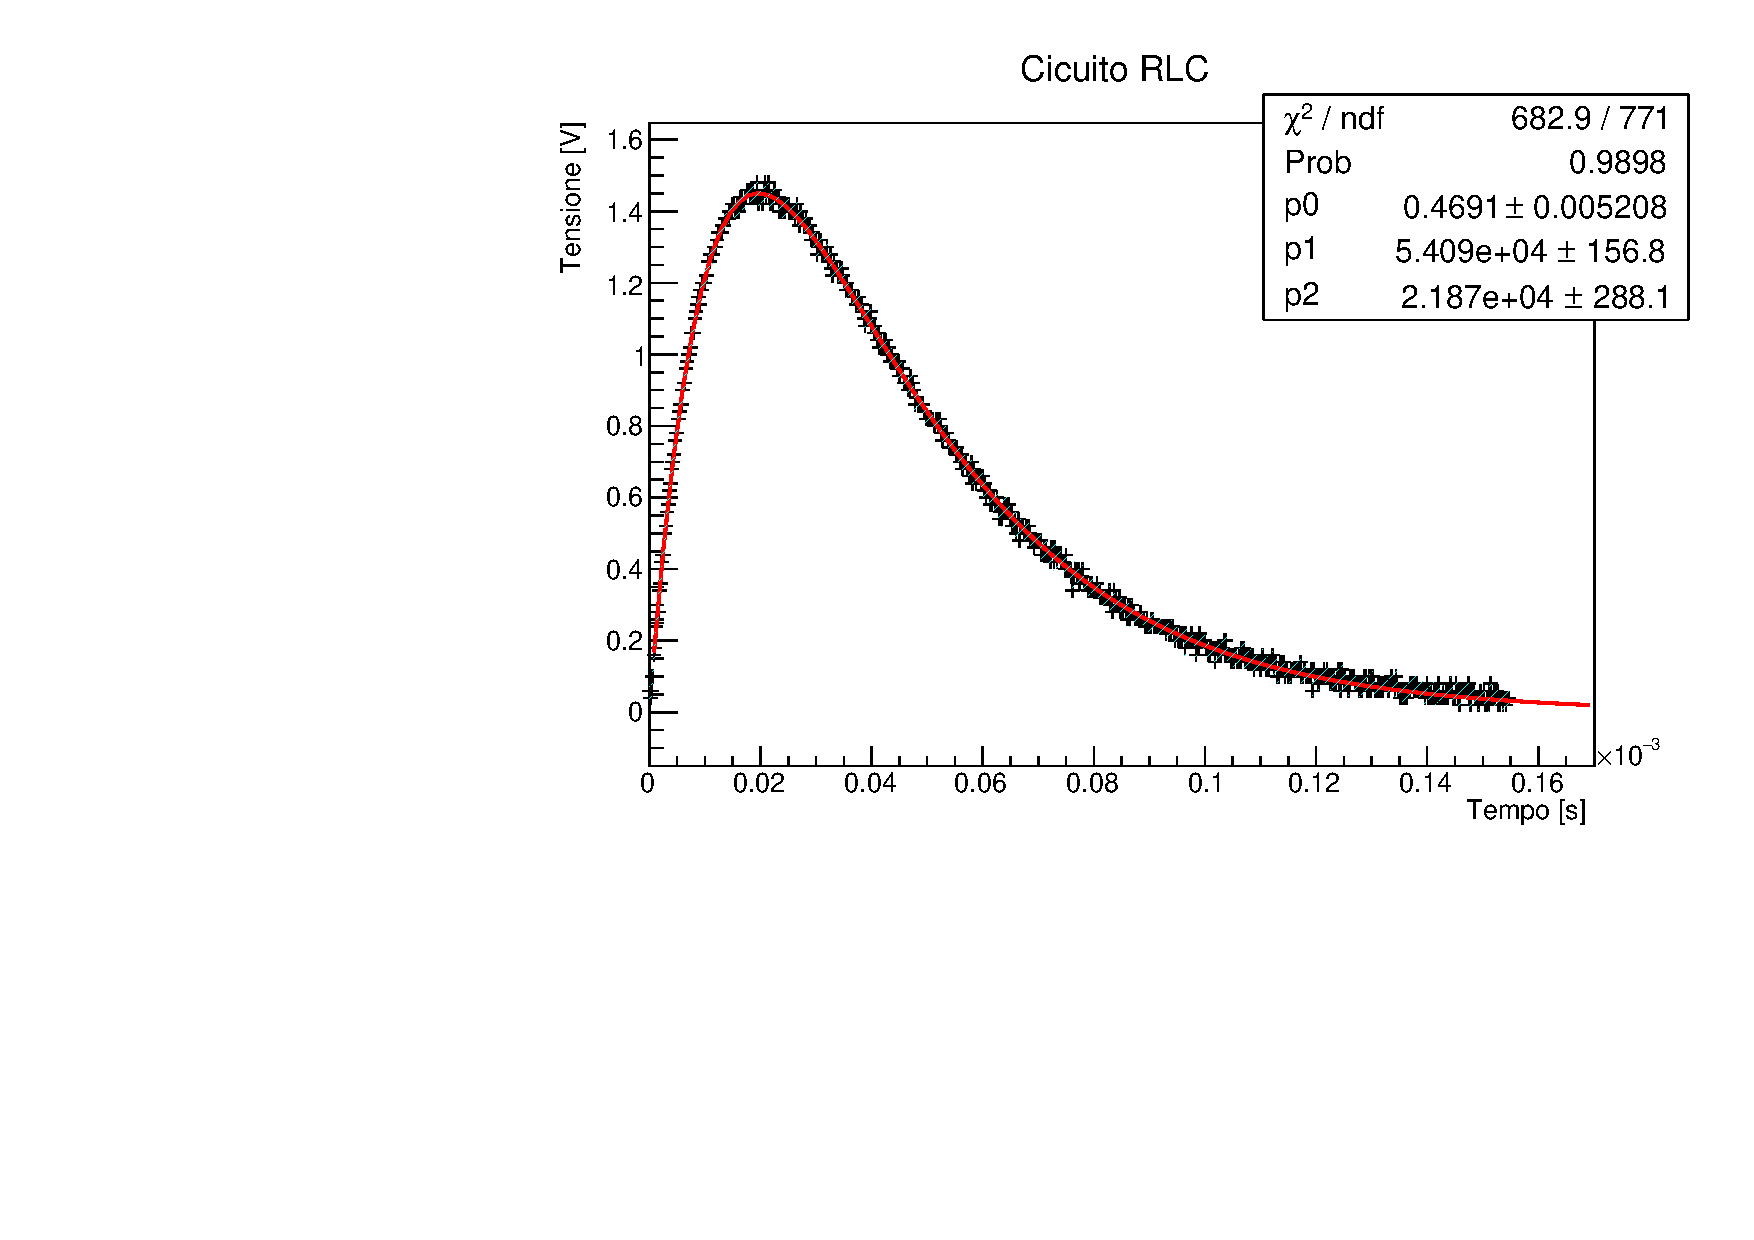
\includegraphics[scale=.4]{Immagini/CircuitoRLC.pdf}
    \caption{Smorzamento critico}
\end{figure}

\begin{table}[H]
    \centering
    \begin{tabular}{cc}
    \toprule
      Parametro   & Valore corrispondente \\
    \midrule
       p0  & $I_0$ \\
       p1  & $\gamma$ \\
       p2  & $\beta$ \\
    \bottomrule
    \end{tabular}
    \caption{}
\end{table}

Si ricava per cui che i parametri di tale circuito sono:
\begin{table}[H]
    \centering
    \begin{tabular}{cc}
        \toprule
      $L (mH)$  & $C(F)\times 10^{-9}$ \\
         \midrule
    $46,21\pm 4,63$     & $8,84\pm 7,57\times 10^{-3}$\\
    \bottomrule
    \end{tabular}
    \caption{}
\end{table}